\section{Architecture}
\label{sec:architecture}

Since the development of a real botnet goes beyond the scope of this work, we adhere to an architecture that allows us to focus on the development of a bot, thought for testing and educational showcase, but actually ready for a real scenario. \Cref{fig:botnet-architecture} shows our botnet reference architecture.

\begin{figure}[tp]
  \centering
  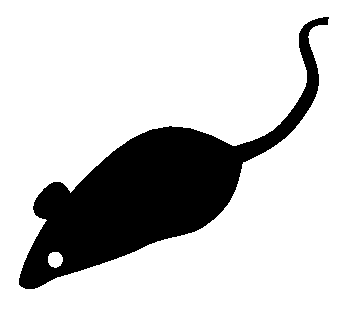
\includegraphics{./fig/acmlarge-mouse}
  \caption{The botnet architecture. In the real scenario, the bot interacts with a web server - e.g. a web server exposing REST APIs. In the testing scenario, the bot mimics the bot-controller interactions, reading/writing local files.}
    \label{fig:botnet-architecture}
\end{figure}

The reference architecture models a bot that can be instructed by a centralized controller.
Here, a controller is defined giving three interfaces: the \textit{init interface} is the one through wich the bot joins the botnet loading specific configuration; the \textit{command interface} is the one through which the bot loads commands to execute; the \textit{log interface} is the one that the bot submits analysis reports to.

Such a model makes our bot is suitable both for local testing, where interfaces are local files, and real bot-controller interaction, where interfaces are REST interfaces. In the following we often says "the bot receives from the controller" and "the bot sends to the controller", meaning that "the bot reads from command interface" and "the bot write to log interface", respectively.

Our bot can be configured by a convenient Web User Interface (WUI) described in \Cref{sec:configuration-wui}. The commands it can execute are given as JSON file. These files can be both local files and remote controller responses. They can be conveniently created by a WUI described in \Cref{sec:commands-wui}.
